
%% Null test is that we perform a fit to data (toy datasets) using SM expectation. 
%% The SM expectation is a flat distribution in which free parameter is an offset (e.g $y = c $).

In this test, 1000 toy datasets generated with SM expection and corresponds 
to Run 2 datase are used. In another words, no signal is injected to these datasets.

Figure~\ref{fig:null_test} show distributions of fit parameters, errors,
$\chi^{2}/ndf$ (ndf is number of degree of freedom) and  $p_{0}$ value of
$\chi^{2}$, from fitting a flat distribution (bkg expection) to the 1000
toy datasets. Since the obserable is a Double Ratio, the fitted off-set (fit parameter)
is allways one in each fit. The normalzed $\chi^{2}$ ($\chi^{2}/ndf$, bottom right plot)
distribution is centered around one which means the toy datasets agree
with a flat distribution (this is what we expected). If we take  $p_0$ > 0.01 as a threshold to determine
if the dataset agree with the SM expectation (flat distribution), then more then 99\% of the toy dataset
passed this cut ($p_0$ > 0.01 ). Since more then 99\% of the samples agree with SM expectation we can conclude
that random fluctuation can not introduce strange shapes that significantly different then a flat distribution.

\begin{figure}[!htb]
  \centering
  \subfloat{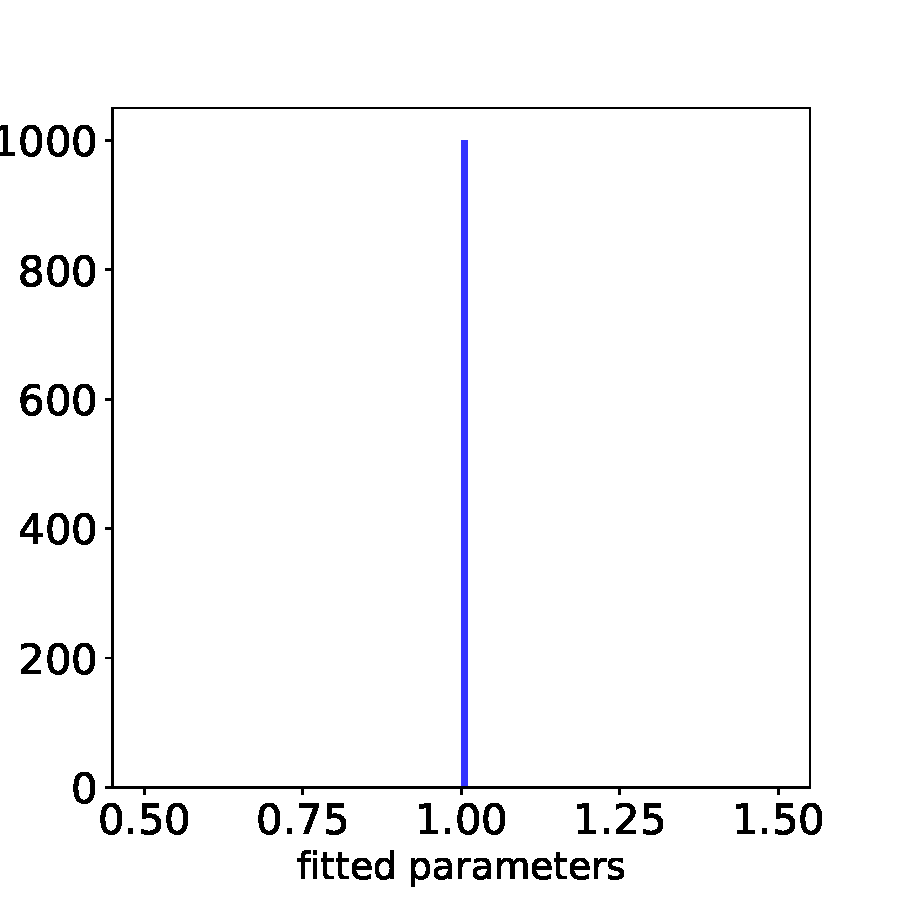
\includegraphics[width=0.40\textwidth]{figs/null_test/Null_test_pars}}
  \subfloat{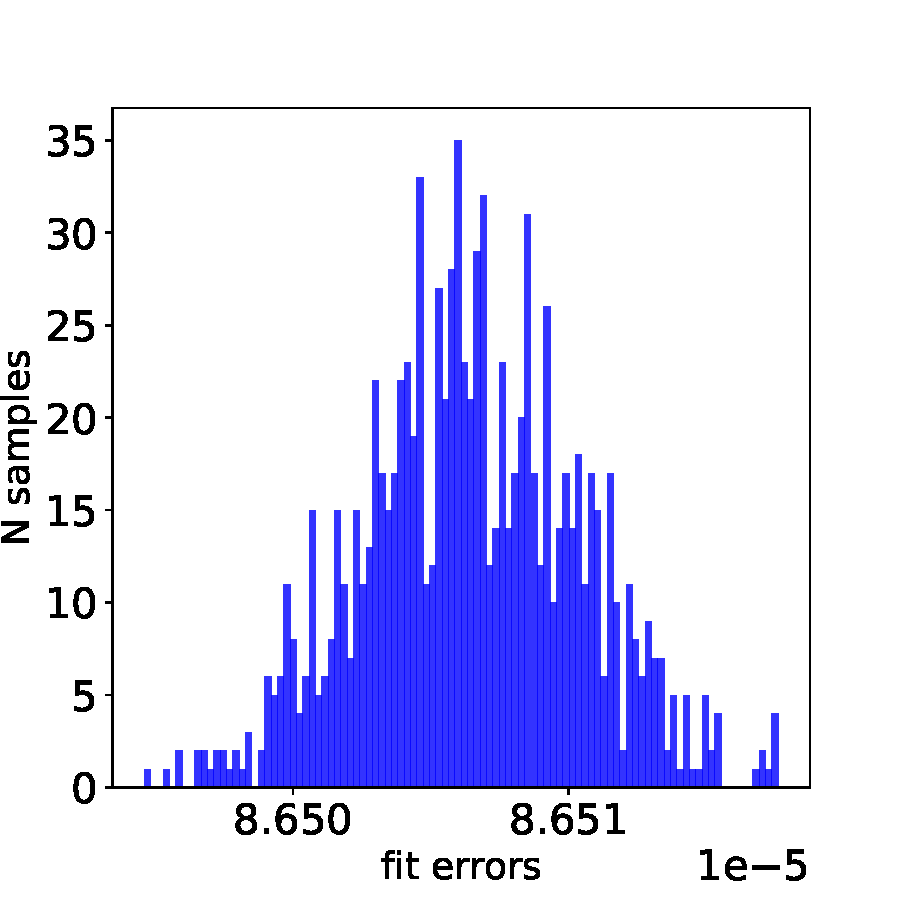
\includegraphics[width=0.40\textwidth]{figs/null_test/Null_test_err}}\\
  \subfloat{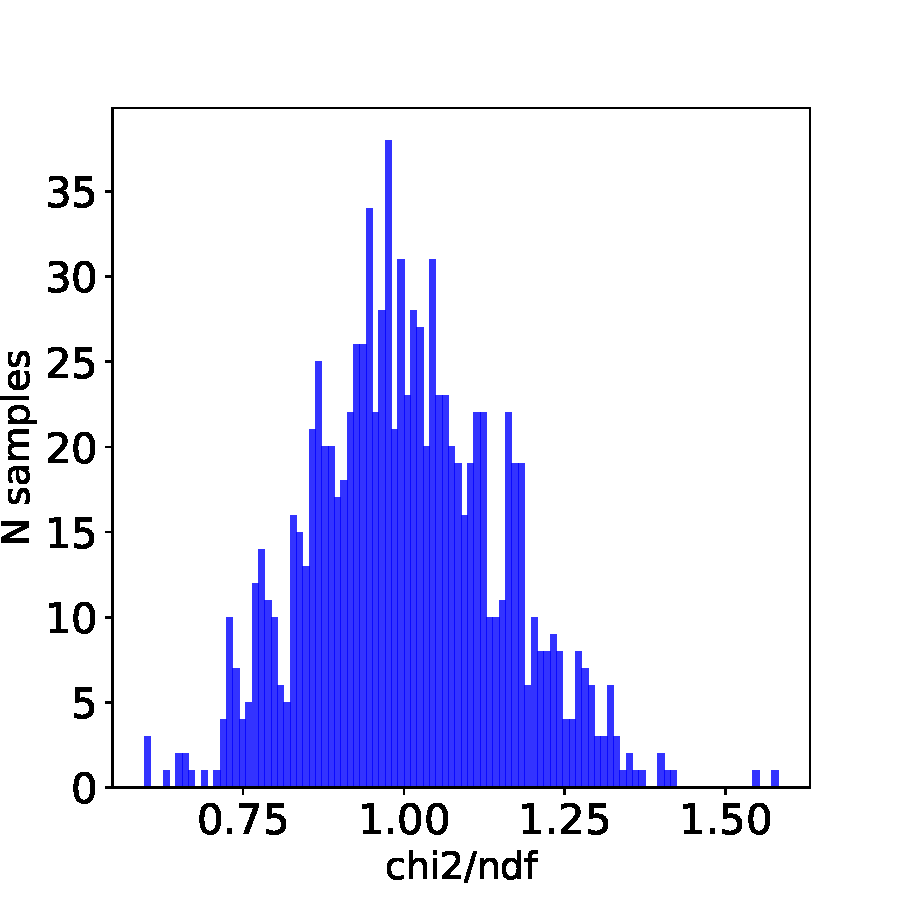
\includegraphics[width=0.40\textwidth]{figs/null_test/Null_test_chi2_ndf}}
  \subfloat{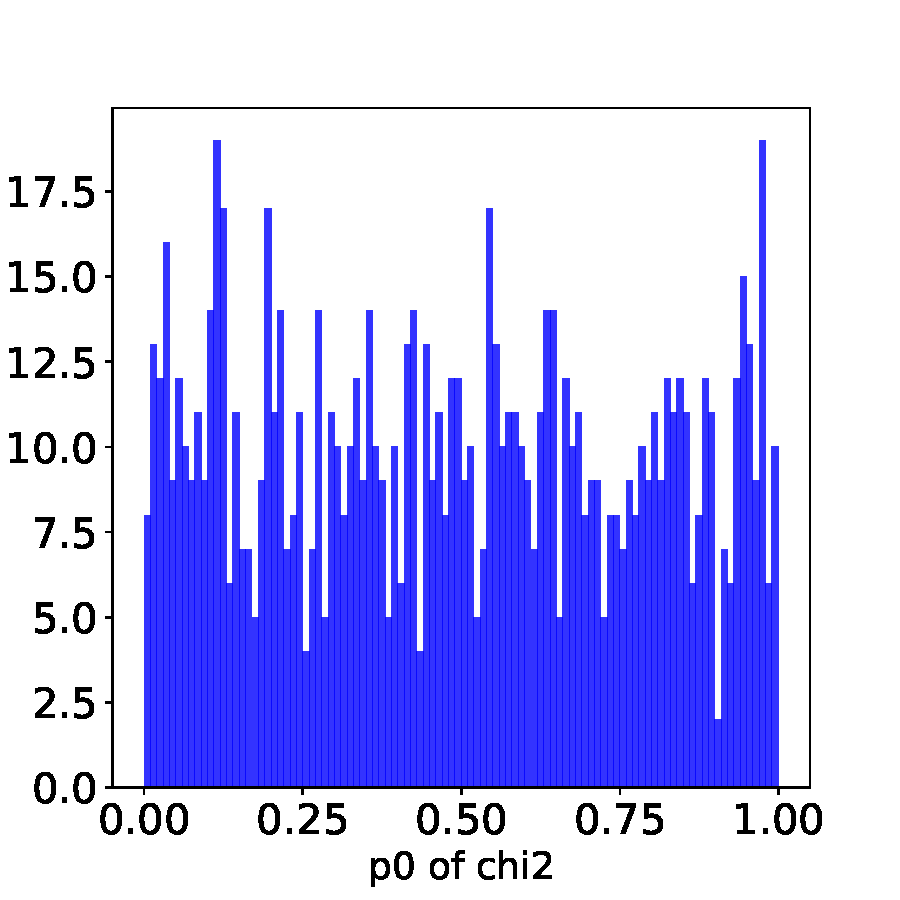
\includegraphics[width=0.40\textwidth]{figs/null_test/Null_test_chi2_p0}}
  \caption{Results of Null Tests on 1000 signal-free toy datasets. Top left plot is estimated parameters, top right is fit errors, bottom left is $\chi^{2}/ndf$ (ndf is number of degree of freedom), bottom right is $p_{0}$ of $\chi^{2}$.}
  \label{fig:null_test}
\end{figure}

